\chapter{Ứng dụng ngôn ngữ Rust}
Để thực hiện ứng dụng ngôn ngữ Rust cho một đối tượng thực tế, tôi chọn đề tài thực hiện ``Hệ thống vườn tưới cây thông minh'' sử dụng kit EK-TM4C123G (hay còn gọi là kit Tiva-C)

\section{Giới thiệu phần cứng}
\subsection{Evaluation kit EK-TM4C123G}
\subsubsection{Giới thiệu kit}
\begin{figure}[ht]
\centering
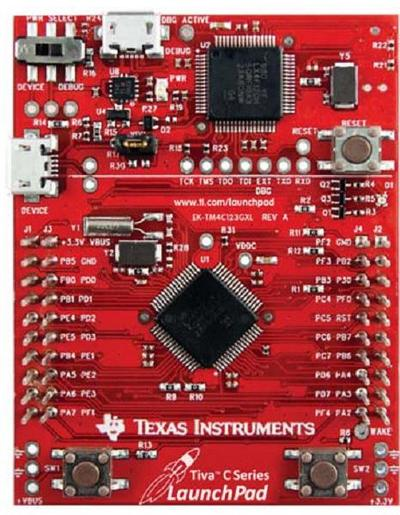
\includegraphics[scale=0.5]{images/kit_tivac.jpg}
\caption{Evaluation kit EK-TM4C123G}
\end{figure}

Evaluation kit EK-TM4C123G (từ đây tôi xin được gọi tắt là kit TIVA C) là một vi điều khiển có kích thước chỉ bằng một thẻ ATM thông dụng.
Kit TIVA C được phát triển bởi tập đoàn Texas Instrument (TI) để thay thế cho sản phẩm Stellaris Launchpad đã dừng sản xuất trước đó.
Dòng TIVA C 32-bit được sử dụng trong đề tài này có một thiết kế hiện đại cùng tập lệnh phong phú và hệ sinh thái về code nhúng giàu có
đã đẩy nhanh việc giảng dạy về lập trình nhúng nói chung trong môi trường trường học cũng như cũng đủ mạnh mẽ để có thể phát triển thêm lên để sử dụng trong môi trường công nghiệp hiện đại.

Kit TIVA C xây dựng xoay quanh bộ xử lý có kiến trúc ARM-Cortex M4F có tốc độ lên đến \si{80\MHz}, có kèm theo bộ tính toán dấu chấm động FPU, nhiều bộ nhớ tích hợp, nhiều chân lập trình GPIO, cũng như nhiều tính năng khác.
Kit TIVA C là một giải pháp hoàn hảo với chi phí thấp để thực hiện những đề tài về lập trình nhúng trong môi trường trường học.

Một số ứng dụng tiêu biểu sử dụng kit TIVA C có thể nêu ra như: xử lý âm thanh giọng nói, điều khiển thiết bị cầm tay, điều khiển nhà thông minh, điều khiển thiết bị y tế, v.v..

Trong đề tài này tôi chọn dòng EK-TM4C123G (cụ thể ở đây là EK-TM4C123GH6PM) là kit phát triển thông dụng nhất của dòng TIVA C được tập đoàn TI sản xuất.

\subsubsection{Thông tin cấu hình kit TIVA C}
\begin{figure}[ht]
\centering
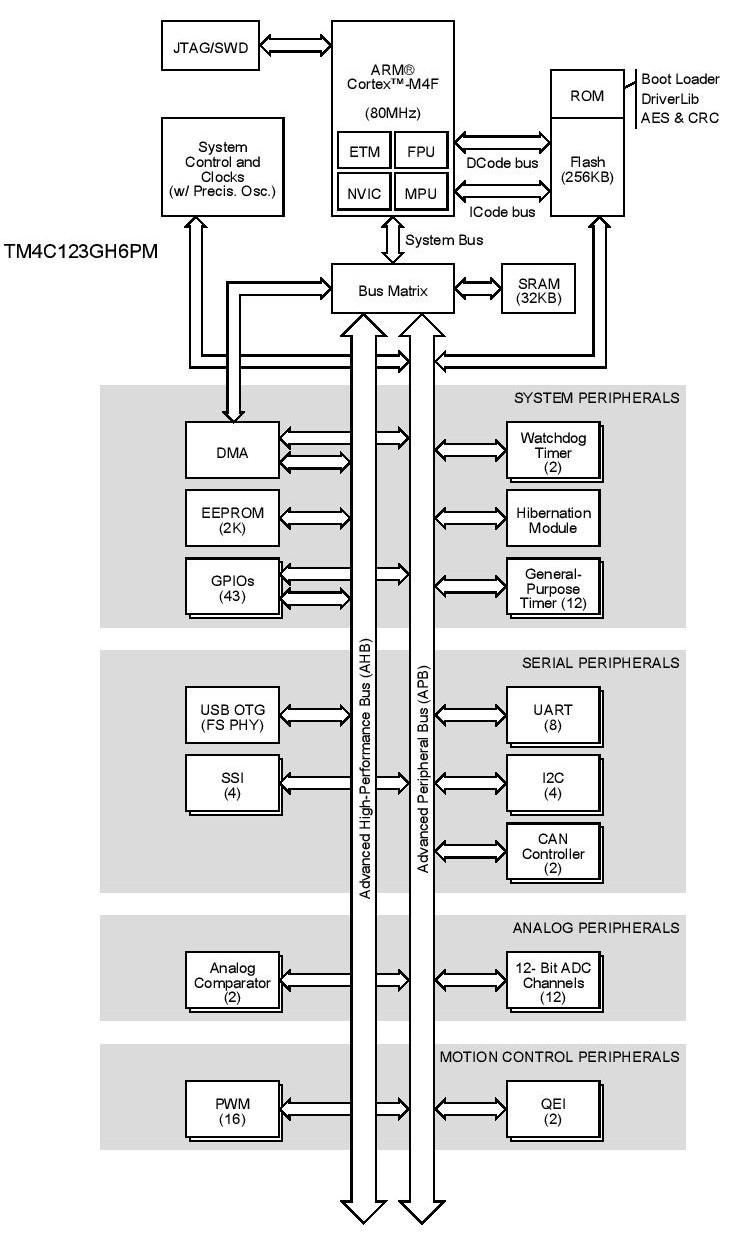
\includegraphics[scale=0.45]{images/tiva_c_diagram.jpg}
\caption{Sơ đồ khối kit TIVA C}
\end{figure}

\textbf{Cấu hình kit TIVA C}
\begin{itemize}
\item Vi xử lý: kiến trúc ARM Cortex-M4F tốc độ lên đến \si{80\MHz} kèm FPU, 100 DMIPS.
\item SRAM: 32KB
\item Bộ nhớ Flash: 256KB
\item EEPROM: 2KB
\end{itemize}

\textbf{Các tính năng nổi bật của kit TIVA C}
\begin{itemize}
\item 6 khối GPIO (A, B, C, D, E, F)
\item 2 modules 12-bit ADC
\item 8 UARTs
\item 4 SSI modules
\item 4 I\textsuperscript{2}C modules
\end{itemize}

\textbf{Ưu điểm}: Giá thành rẻ, nhỏ gọn, mạnh mẽ. Có bộ thư viện phong phú dễ dàng thực hiện lập trình nhúng trên nhiều lĩnh vực.
Khả năng hoạt động với chế độ tiết kiệm điện để hoạt động liên tục, phù hợp cho việc áp dụng cho môi trường thực tiễn.

\textbf{Nhược điểm}: Giá thành vẫn còn đắt hơn so với một số thiết bị dòng STM32, không có tích hợp GPU nên rất khó để lập trình nhúng liên quan đến xử lý ảnh nói chung.

\pagebreak
\textbf{Thông số LCD 1602}:
\begin{itemize}
\item Điện áp MAX: \si{7\volt}
\item Điện áp MIN: \si{\num{-0.3}\volt}
\item Điện áp hoạt động: \SIrange[range-phrase=--, range-units=single]{2.7}{5.5}{\volt}
\item Dòng điện cấp nguồn: \SIrange[range-phrase=--, range-units=single]{350}{600}{\micro\ampere}
\item Nhiệt độ hoạt động: \SIrange[range-phrase=--, range-units=single]{-30}{75}{\celsius}
\end{itemize}

\begin{longtable}{l l p{0.7\textwidth}} \toprule
Chân & Ký hiệu & Mô tả \\
\midrule
\endhead
1 & VSS & Chân nối đất cho LCD, khi thiết kế mạch nối chân này với GND của mạch điều khiển \\ \midrule
2 & VDD & Chân cấp nguồn cho LCD, khi thiết kế mạch nối chân này với chân cấp nguồn \si{5\volt} của mạch điều khiển \\ \midrule
3 & V0 & Điều chỉnh độ tương phản của LCD \\ \midrule
4 & RS & Chân chọn thanh ghi (Register Select). Nối chân RS với logic ``0'' (GND) hoặc logic ``1'' (VCC) để chọn thanh ghi.\newline
- Logic ``0'': Bus DB0--DB7 sẽ nối với thanh ghi lệnh IR của LCD (ở chế độ ``ghi'' - write) hoặc nối với bộ đếm địa chỉ của LCD (ở chế độ ``đọc'' - read)\newline
- Logic ``1'': Bus DB0--DB7 sẽ nối với thanh ghi dữ liệu bên trong LCD. \\ \midrule
5 & R/W & Chân chọn chế độ đọc/ghi (read/write). Nối chân R/W với logic ``0'' để LCD hoạt động ở chế độ ghi, hoặc nối với logic ``1'' để LCD hoạt động ở chế độ đọc. \\ \midrule
6 & E & Chân cho phép hoạt động (Enable). Sau khi các tín hiệu được đặt lên bus DB0--DB7, các lệnh chỉ được chấp nhận khi có 1 xung cho phép của chân E.\newline
- Ở chế độ ghi: Dữ liệu ở bus sẽ được LCD chuyển vào (chấp nhận) thanh ghi bên trong nó khi phát hiện một cạnh xuống (high-to-low transistion) của tín hiệu E.\newline
- Ở chế độ đọc: Dữ liệu sẽ được LCD xuất ra DB0--DB7 khi phát hiện cạnh lên (low-to-high transistion) ở chân E và được LCD giữ ở bus đến khi nào chân E xuống mức thấp. \\ \midrule
7--14 & DB0--DB7 & 8 đường của bus dữ liệu dùng để trao đổi thông tin với mạch điều khiển. Có 2 chế độ sử dụng 8 đường bus này:\newline
- Chế độ 8-bit: Dữ liệu được truyền trên cả 8 đường, với MSB là bit DB7.\newline
- chế độ 4-bit: Dữ liệu được truyền hai lần trên 4 đường DB4--DB7, với bit MSB là DB7. \\ \midrule
15 & --- & Nguồn cấp cho đèn nền của LCD. \\ \midrule
16 & --- & Chân GND cho đèn nền của LCD. \\
\bottomrule
\caption{Chức năng các chân của LCD 1602}
\end{longtable}
\textbf{Ghi chú}:\newline
Ở chế độ ``đọc'', nghĩa là mạch điều khiển đọc thông tin từ LCD thông qua các chân DBx.
Còn khi ở chế độ ``ghi'', nghĩa là mạch điều khiển xuất thông tin điều khiển cho LCD thông qua các chân DBx.

\subsubsection{Các chân điều khiển việc đọc ghi vào LCD 1602}
\begin{itemize}
    \item \textbf{RS (chân số 3)}:
\end{itemize}
Chân lựa chọn thanh ghi (Select Register), chân này cho phép lựa chọn 1 trong 2 thanh ghi IR hoặc DR để làm việc.
Vì cả 2 thanh ghi này đều được kết nối với các chân Data của LCD nên cần 1 bit để lựa chọn giữa chúng.
Nếu \(RS = 0\), thanh ghi IR được chọn và nếu \(RS = 1\) thanh ghi DR được chọn.

Chúng ta đều biết thanh ghi IR là thanh ghi chứa mã lệnh cho LCD,
vì thế nếu muốn gởi 1 mã lệnh đến LCD thì chân RS phải được reset về 0.
Ngược lại, khi muốn ghi mã ASCII của ký tự cần hiển thị lên LCD thì chúng ta sẽ set \(RS = 1\) để chọn thanh ghi DR.
\begin{itemize}
    \item \textbf{R/W (chân số 4)}:
\end{itemize}
Chân lựa chọn giữa việc đọc và ghi.
Nếu \(R/W = 0\) thì dữ liệu sẽ được ghi từ mạch điều khiển vào LCD.
Nếu \(R/W = 1\) thì dữ liệu sẽ được đọc từ LCD ra ngoài.
Tuy nhiên, chỉ có duy nhất 1 trường hợp mà dữ liệu có thể đọc từ LCD ra,
đó là đọc trạng thái LCD để biết LCD có đang bận hay không \emph{cBusyFlag - BF} .
Do LCD là một thiết bị hoạt động tương đối chậm (so với vi điều khiển),
vì thế một cờ BF được dùng để báo LCD đang bận, nếu \(BF = 1\) thì chúng ta phải chờ cho LCD xử lí xong nhiệm vụ hiện tại,
đến khi nào \(BF = 0\) một thao tác mới sẽ được gán cho LCD.
Vì thế, khi làm việc với Text LCD chúng ta nhất thiết phải có một chương trình con nào đó để chờ cho đến khi LCD rảnh.

Có 2 cách để viết chương trình \emph{waitLCD}.
Cách 1 là đọc bit BF về kiểm tra và chờ \(BF = 0\),
cách này đòi hỏi lệnh đọc từ LCD về bộ điều khiển ngoài, do đó chân R/W cần được nối với bộ điều khiển ngoài.
Cách 2 là viết một hàm delay một khoảng thời gian cố định nào đó. %(tốt nhất là trên \si{1\ms}).
Ưu điểm của cách 2 là sự đơn giản vì không cần đọc LCD, do đó chân R/W không cần sử dụng và luôn được nối với GND.
Tuy nhiên, nhược điểm của cách 2 là khoảng thời gian delay cố định nếu quá lớn sẽ làm chậm quá trình thao tác LCD,
nếu quá nhỏ sẽ gây ra lỗi hiển thị.
\begin{itemize}
    \item \textbf{E (chân số 5)}:
\end{itemize}
Chân cho phép LCD hoạt động (Enable), chân này cần được kết nối với bộ điều khiển để cho phép thao tác LCD.
Để đọc và ghi data từ LCD chúng ta cần tạo một xung cạnh xuống trên chân EN,
nói theo cách khác, muốn ghi dữ liệu vào LCD trước hết cần đảm bảo rằng chân \(EN = 0\),
tiếp đến xuất dữ liệu đến các chân DB0 đến DB7, sau đó set chân EN lên 1 và cuối cùng là xóa EN về 0 để tạo 1 xung cạnh xuống.
